\section{Analyse technique}
	Cette section est destinée à détailler les techniques mises en œuvres afin d'implémenter les différentes fonctionnalités décrites dans la section précédente. Le but de cette analyse technique est de montrer le raisonnement qui a conduit à la structure actuelle de notre générateur de contenu statique. Nous n'exposerons donc pas les détails d'implémentations. Si cela vous intéresse, le code source à disposition sur \url{https://github.com/MaximeDeWolf/DGSC/tree/master/code/src}.
	
	\subsection{Règles}
	%todo trouver un autre nom pour "target" qui suggère une entrée
	%todo mieux expliquer ce que désigne les champs d'une règle + exemple
	
	Une règle de génération est le moyen que nous mettons à disposition à l' utilisateur pour que celui-ci spécifie à notre générateur de contenu statique pour désigner le comportement que celui-ci doit adopter.
	Typiquement, une règle représente un cas d'utilisation. Il s'agit donc d'un des points les plus importants du projet. Cette sous-section explique donc en détail les différents éléments qui définissent ces règles ainsi que leur structure.
	
	\subsubsection*{Le format}
	
		Le format des fichiers de règles se doit de posséder deux qualités importantes. La première est d'être facilement compréhensible par l'utilisateur aussi bien lors de la lecture que de l'écriture. La deuxième est de pouvoir être analysé facilement par notre générateur de contenu statique dans le but d'y lire les informations nécessaire à son fonctionnement.
		
		Nous avons donc choisis le format \textit{YAML} pour stocker ces règles. Chaque fichier de règles contient donc une liste de règles. Ces règles contiennent chacune quatre champs qui eux-mêmes contiennent une expression. Ce sont ces expressions qui seront évaluées par notre générateur. La Figure \ref{fig:rule:format} illustre le format type d'un fichier de règles.
		
		\begin{figure}[!]
			\centering
			\lstinputlisting[inputencoding=utf8/latin1]{codeSample/ruleFormat.yaml}
			\caption{Format d'un fichier de règles de notre générateur}
			\label{fig:rule:format}
		\end{figure}
		
	\subsubsection*{Les expressions}
	
	\subsubsection*{Les champs}
		Ces règles possèdent quatre champs obligatoires: \textit{target}, \textit{template}, \textit{data} et \textit{output}. Comme expliqué dans la précédente section, chacun de ces champs (ou ensemble de champs) permet de  contrôler les paramètres de notre générateur. \textit{target} et \textit{output} représentent le contenudu générateur tandis que \textit{template} et \textit{data} représentent respectivement le \textit{template} et les données. Les particularités et fonctions de chacun de ces champs sont expliqués ci-dessous.
		
		
		\subsubsection*{Target}
			Le champ \textit{target} contient une expression destinée à être lue par notre générateur. Le résultat de cette expression sert à définir la multiplicité du paramètre "contenu" de la règle. Cela définit le nombre de fois que les autres champs de la règles courantes doivent être évalués. A chaque itération de ce processus un \textit{item} différent est stocké dans une variable appelée \textit{current}. Cette variable est ensuite utilisable dans les autres champs de la règle courante.
		
		\subsubsection*{Template}
		%todo clarifier quel moteur de template gère le cas MultiTemplatesIn
			Ce champs contient une expression destinée à être évaluée par notre générateur de contenu statique. Le résultat de cette expression à désigner le \textit{template} à utiliser sur les données chargées grâce au champ \textit{data}.\\
			
			La multiplicité de ce paramètre est volontairement bloquée à un. En effet, cela simplifie ainsi l'utilisation de notre générateur de contenu statique bien cela limite également souplesse d'utilisation. Cette limitation nous empêche de réaliser les cas d'utilisation \textbf{ManyTemplatesIn} et \textbf{ManyTemplateOut}. Nous avons toutefois montré un moyen de contourner cette limitation dans la Section 2.
		
		\subsubsection*{Data}
			Ce champs contient un ensemble de paires clés/valeurs. Chacune de ces valeurs est une expression destinée à être évaluée par notre générateur de contenu statique. Chaque clé de cette ensemble devient une variable dont la valeur est le résultat de son expression évaluée par notre générateur. Ces variables sont par la suite utilisables dans le \textit{template} sélectionné par le champ \textit{template}. La multiplicité de ce champs définit la multiplicité du paramètre "données" du cas d'utilisation. 
		
		\subsubsection*{Output}
			Ce champ contient une expression destinée à être évaluée par notre générateur de contenu statique. Le résultat de cette expression désigne le chemin vers le fichier où le résultat final de l'application du \textit{template} sur les données doit être écrit. Ce champs influence indirectement la multiplicité de paramètre "contenu" du cas d'utilisation. En effet, même si la multiplicité de ce paramètre est sensée être supérieure à un, fournir à tous ces \textit{items} de contenu le même fichier de sortie entraîne l'écrasement de ceux-ci pour au final ne contenir que le dernier \textit{item} généré.
	
	
	\subsection{Structure}
	%todo détailler et expliquer le diagramme de classe
		Comme mentionné dans la Section 4, nous appliquons la programmation modulaire afin de permettre une grande flexibilité à notre générateur de contenu statique. Nous avons donc conçu l'architecture dans cette optique comme le montre la Figure \ref{fig:class_diagram}. Un utilisateur pourra donc modifier le comportement de notre générateur en implémentant lui même l'une de ces interfaces. Il pourra, entre autres, modifier la syntaxe des règles mentionnées ci-dessus en implémentant l'interface \textit{RuleBackend}.
		
		Comme expliqué dans la section précédente, nous fournirons par défaut une implémentation de ces interfaces qui permettra à l'utilisateur de réaliser les cas d'utilisations listés en Section 2.
		
		\begin{figure}
			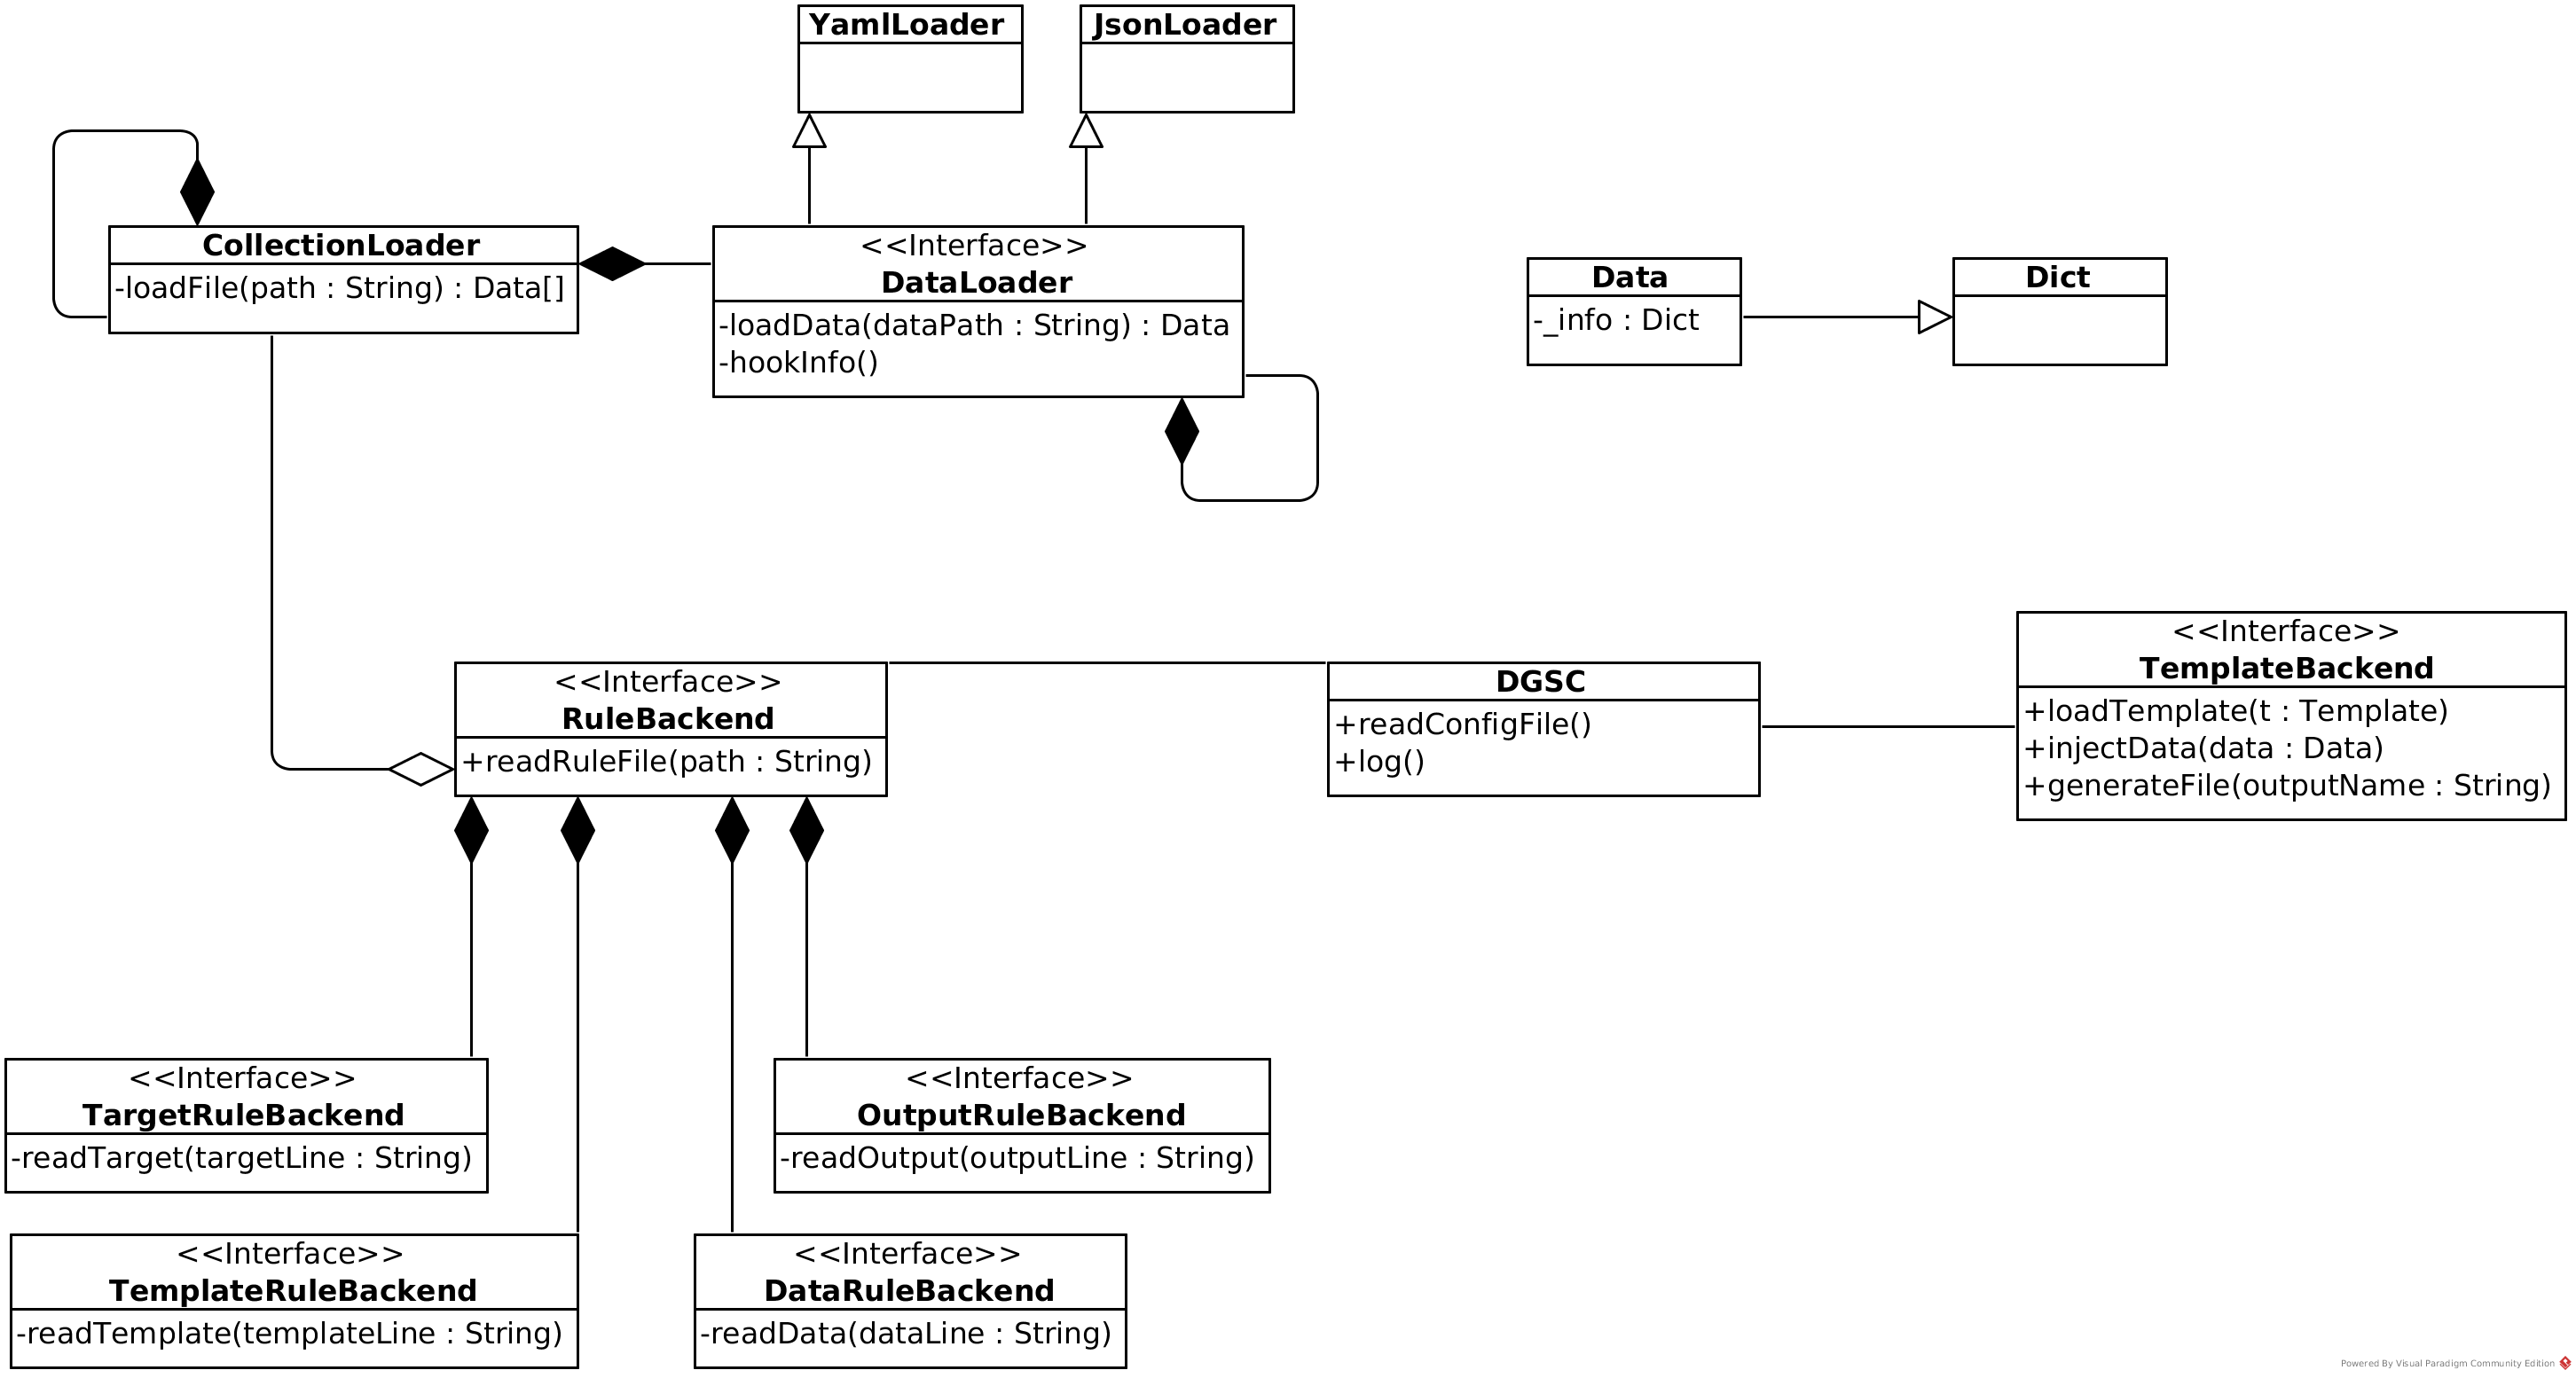
\includegraphics[width=\textwidth]{/diagrams/DGSC}
			\caption{Diagramme de classes de notre générateur de contenu statique}
			\label{fig:class_diagram}
		\end{figure} 
	
	
	\subsection{Configuration}
		Un fichier de configuration permettra à l'utilisateur de spécifier quelques options à notre générateur de contenu statique. Parmi ces options, nous retrouverons entre autres: le répertoire de travail en entrée, le répertoire de travail en sortie, une liste de classes implémentant les interfaces du générateur, l'emplacement du fichier de \textit{logs} (le cas échéant), ... Chacune de ses options aura une valeur par défaut, l'utilisateur ne devra donc spécifier que les éléments qui diffèrent de la configuration par défaut. 